% PREÁMBULO
\documentclass[letterpaper]{article}
\usepackage[utf8]{inputenc}
\usepackage[spanish]{babel}

\usepackage{enumitem}
\usepackage{titling}

% Símbolos
	\usepackage{amsmath}
	\usepackage{amssymb}
	\usepackage[utf8]{inputenc}
	\usepackage[T1]{fontenc}
	\usepackage{mathtools}
	\usepackage{multicol}
	\usepackage[thinc]{esdiff}

% Márgenes
	\usepackage
	[
		margin = 1.4in
	]
	{geometry}

% Imágenes
	\usepackage{float}
	\usepackage{graphicx}
	\graphicspath{{imagenes/}}
	\usepackage{subcaption}

% Ambientes
	\usepackage{amsthm}

	\theoremstyle{definition}
	\newtheorem{ejercicio}{Ejercicio}

	\newtheoremstyle{lemathm}{4pt}{0pt}{\itshape}{0pt}{\bfseries}{ --}{ }{\thmname{#1}\thmnumber{ #2}\thmnote{ (#3)}}
	\theoremstyle{lemathm}
	\newtheorem{lema}{Lema}

	\newtheoremstyle{lemademthm}{0pt}{10pt}{\itshape}{ }{\mdseries}{ --}{ }{\thmname{#1}\thmnumber{ #2}\thmnote{ (#3)}}
	\theoremstyle{lemademthm}
	\newtheorem*{lemadem}{Demostración}

% Ajustes
	\allowdisplaybreaks	% Los align pueden cambiar de página

% Macros
	\newcommand{\sumi}[2]{\sum_{i=#1}^{#2}}
	\newcommand{\dint}[2]{\displaystyle\int_{#1}^{#2}}
	\newcommand{\inte}[2]{\int_{#1}^{#2}}
	\newcommand{\dlim}{\displaystyle\lim}
	\newcommand{\limxinf}{\lim_{x\to\infty}}
	\newcommand{\limninf}{\lim_{n\to\infty}}
	\newcommand{\dlimninf}{\displaystyle\lim_{n\to\infty}}
	\newcommand{\limh}{\lim_{h\to0}}
	\newcommand{\ddx}{\dfrac{d}{dx}}
	\newcommand{\txty}{\text{ y }}
	\newcommand{\txto}{\text{ o }}
	\newcommand{\Txty}{\quad\text{y}\quad}
	\newcommand{\Txto}{\quad\text{o}\quad}
	\newcommand{\si}{\text{si}\quad}

	\newcommand{\etiqueta}{\stepcounter{equation}\tag{\theequation}}
	\newcommand{\tq}{:}
	\renewcommand{\o}{\circ}
	% \newcommand*{\QES}{\hfill\ensuremath{\boxplus}}
	% \newcommand*{\qes}{\hfill\ensuremath{\boxminus}}
	% \newcommand*{\qeshere}{\tag*{$\boxminus$}}
	% \newcommand*{\QESHERE}{\tag*{$\boxplus$}}
	\newcommand*{\QES}{\hfill\ensuremath{\blacksquare}}
	\newcommand*{\qes}{\hfill\ensuremath{\square}}
	\newcommand*{\QESHERE}{\tag*{$\blacksquare$}}
	\newcommand*{\qeshere}{\tag*{$\square$}}
	\newcommand*{\QED}{\hfill\ensuremath{\blacksquare}}
	\newcommand*{\QEDHERE}{\tag*{$\blacksquare$}}
	\newcommand*{\qel}{\hfill\ensuremath{\boxdot}}
	\newcommand*{\qelhere}{\tag*{$\boxdot$}}
	\renewcommand*{\qedhere}{\tag*{$\square$}}

	\newcommand{\abs}[1]{\left\vert#1\right\vert}
	\newcommand{\suc}[1]{\left(#1_n\right)_{n\in\N}}
	\newcommand{\en}[2]{\binom{#1}{#2}}
	\newcommand{\upsum}[2]{U(#1,#2)}
	\newcommand{\lowsum}[2]{L(#1,#2)}

	\newcommand{\N}{\mathbb{N}}
	\newcommand{\Q}{\mathbb{Q}}
	\newcommand{\R}{\mathbb{R}}
	\newcommand{\Z}{\mathbb{Z}}
	\newcommand{\eps}{\varepsilon}
	\newcommand{\ttF}{\mathtt{F}}
	\newcommand{\bfF}{\mathbf{F}}

	\newcommand{\To}{\longrightarrow}
	\newcommand{\mTo}{\longmapsto}
	\newcommand{\ssi}{\Longleftrightarrow}
	\newcommand{\sii}{\Leftrightarrow}
	\newcommand{\then}{\Rightarrow}

	\newcommand{\pTFC}{{\itshape 1er TFC\/}}
	\newcommand{\sTFC}{{\itshape 2do TFC\/}}

%Code

	\usepackage{listings}
	\usepackage{xcolor}
	\lstset { %
		language=C++,
		backgroundcolor=\color{black!5}, % set backgroundcolor
		basicstyle=\footnotesize,% basic font setting
		breaklines=true
		postbreak=\mbox{\textcolor{red}{$\hookrightarrow$}\space}
	}

% Membrete
	\usepackage{fancyhdr}
	\setlength{\headheight}{14pt}
	\pagestyle{fancy}
	\fancyhf{}
	\rhead{\theauthor}
	\lhead{\thetitle}
	\cfoot{\thepage}

% Datos
    \title{Cálculo II\\Examen II}
    \author{Rubén Pérez Palacios\\Profesor: Dr. Fernando Nuñez Medina}
    \date{30 Abril 2020}

% DOCUMENTO
\begin{document}
	\maketitle

	\section*{Problemas}

	\begin{enumerate}
		\item Esturcturas de datos, selecciona la adecuadda.
		\begin{enumerate}
			\item Cola, requieres de una escturctura donde puedas a acceder a ellos en la forma en que fueron agregados desde el primero hasta el último es decir $FIFO$ la definición de cola.
			\item Arreglo no ordenado, ya que permite el acceso aleatorio de sus elementos en $O(1)$-
			\item Pila, requieres de una escturctura donde puedas a acceder a ellos en la forma en que fueron agregados desde el último hasta el primero es decir $FILO$ la definición de pila.
			\item Set, ya que este como nos permitira acceder, borrar e insertar en $O(logN)$. De las opciones la mejor es la lista doblemente ligada ya que nos permite una manejo de memoria flexible, pero el acceder, agregar y eleminar sus elementos es en $O(N)$ por lo que sería lento.
			\item Lista doblemente ligada $dequeue$, esta te permite flexibilidad en el tamaño y memeria de los datos, y permite acceder e insertar al inicio y al final de esta.
		\end{enumerate}
		\item Pila
		\begin{enumerate}
			\item Creamos un arreglo del tamaño máximo de la pila, y guardamos la posición del último elemento insertado en el pila (o ínidicamos que no hay ninguno). Al insertar un elemento lo guardamos en la siguiente posición del úlitmo elemento insertado, y al eliminar borramos el último elemento insertado y para ambos actualizamos la posición del último elemento insertado.
			\item Creamos una lista simplemente ligada y una apuntador que indicara el primer elemento. Al agregar un elemento lo hacemos al final en nuestra lista, y al quitar solo movemos nuestro apuntador al nodo que apunta el nodo al que estabamos apuntando
			\item Creamos dos colas, una para guardar los elementos de la pila (digamos stack), y otra para efectuar (digamos tmp). Al agregar un elemento, lo agregamos a la cola tmp, y despues movemos uno por uno los elemntos de stack a tmp y por último regresamos todos los elementos a tmp; para quitar un elemento, moevemos todos los elementos de stack a tmp, hacemos pop en tmp y regresamos todos los elementos a stack.
		\end{enumerate}
		\newpage
		\item Cola
		\begin{enumerate}
			\item Creamos un arreglo del tamaño máximo de la pila, y guardamos la posición del último elemento insertado en el pila (o ínidicamos que no hay ninguno), a diferencia de la cola en el arreglo los iremos agregando de final a inicio. Al insertar un elemento lo guardamos en la anterior posición del úlitmo elemento insertado, y al eliminar borramos el último elemento insertado y para ambos actualizamos la posición del último elemento insertado.
			\item Creamos una lista simplemente ligada. Al agregar y al quitar un elemento lo hacemos al final en nuestra lista.
			\item Tenemos dos pilas. La principal, y la ayuda. En la principal guardamos la cola. Para agregar un numero, solo lo agregamos a la pila principal. Para quitar un numero, pasamos todos los numeros de la pila principal, a la de ayuda, exceptuando el ultimo numero. Y ahora regresamos los numeros de la pila principal a la de ayuda.
		\end{enumerate}
		\item POO
		
		\begin{enumerate}
			\item Código corregido
			
			\begin{lstlisting}
			
#include"iostream"
using namespace std;
class Vector3
{
	private :
		float x,y,z;
	public :
		Vector3 ( float x0 , float y0 , float z0 ) 
		{
			x=x0; 
			y=y0; 
			z=z0;
		}
		void imprime () 
		{
			cout<<x<<" "<<y<<" "<<z<<'$\setminus$n';
		}
		float getX(){ return x;}
		float getY(){ return y;}
		float getZ(){ return z;}
		float setX(float tmp){ return x = tmp;}
		float setY(float tmp){ return y = tmp;}
		float setZ(float tmp){ return z = tmp;}
};
Vector3* sumaVectores ( Vector3 *a, Vector3 *b)
{
	return *ret = new Vector3(a->getX()+b->getX(),a->getY()+b->getY(),a->getZ()+b->getZ()) ;
}

int main () {
	Vector3 v1(1 ,2 ,3) ;
	Vector3 v2(4 ,5 ,6) ;
	Vector3 *suma=sumaVectores (&v1,&v2) ;
	suma->imprime();
	delete suma;
	return 0;
}

			\end{lstlisting}

			\item Separar la definicion de la clase en una librería aparte y sobrecargar el operador +.
		\end{enumerate}
		
		\item Heap
		
		\begin{multicols}{2}

			\begin{figure}[H]
				\centering
				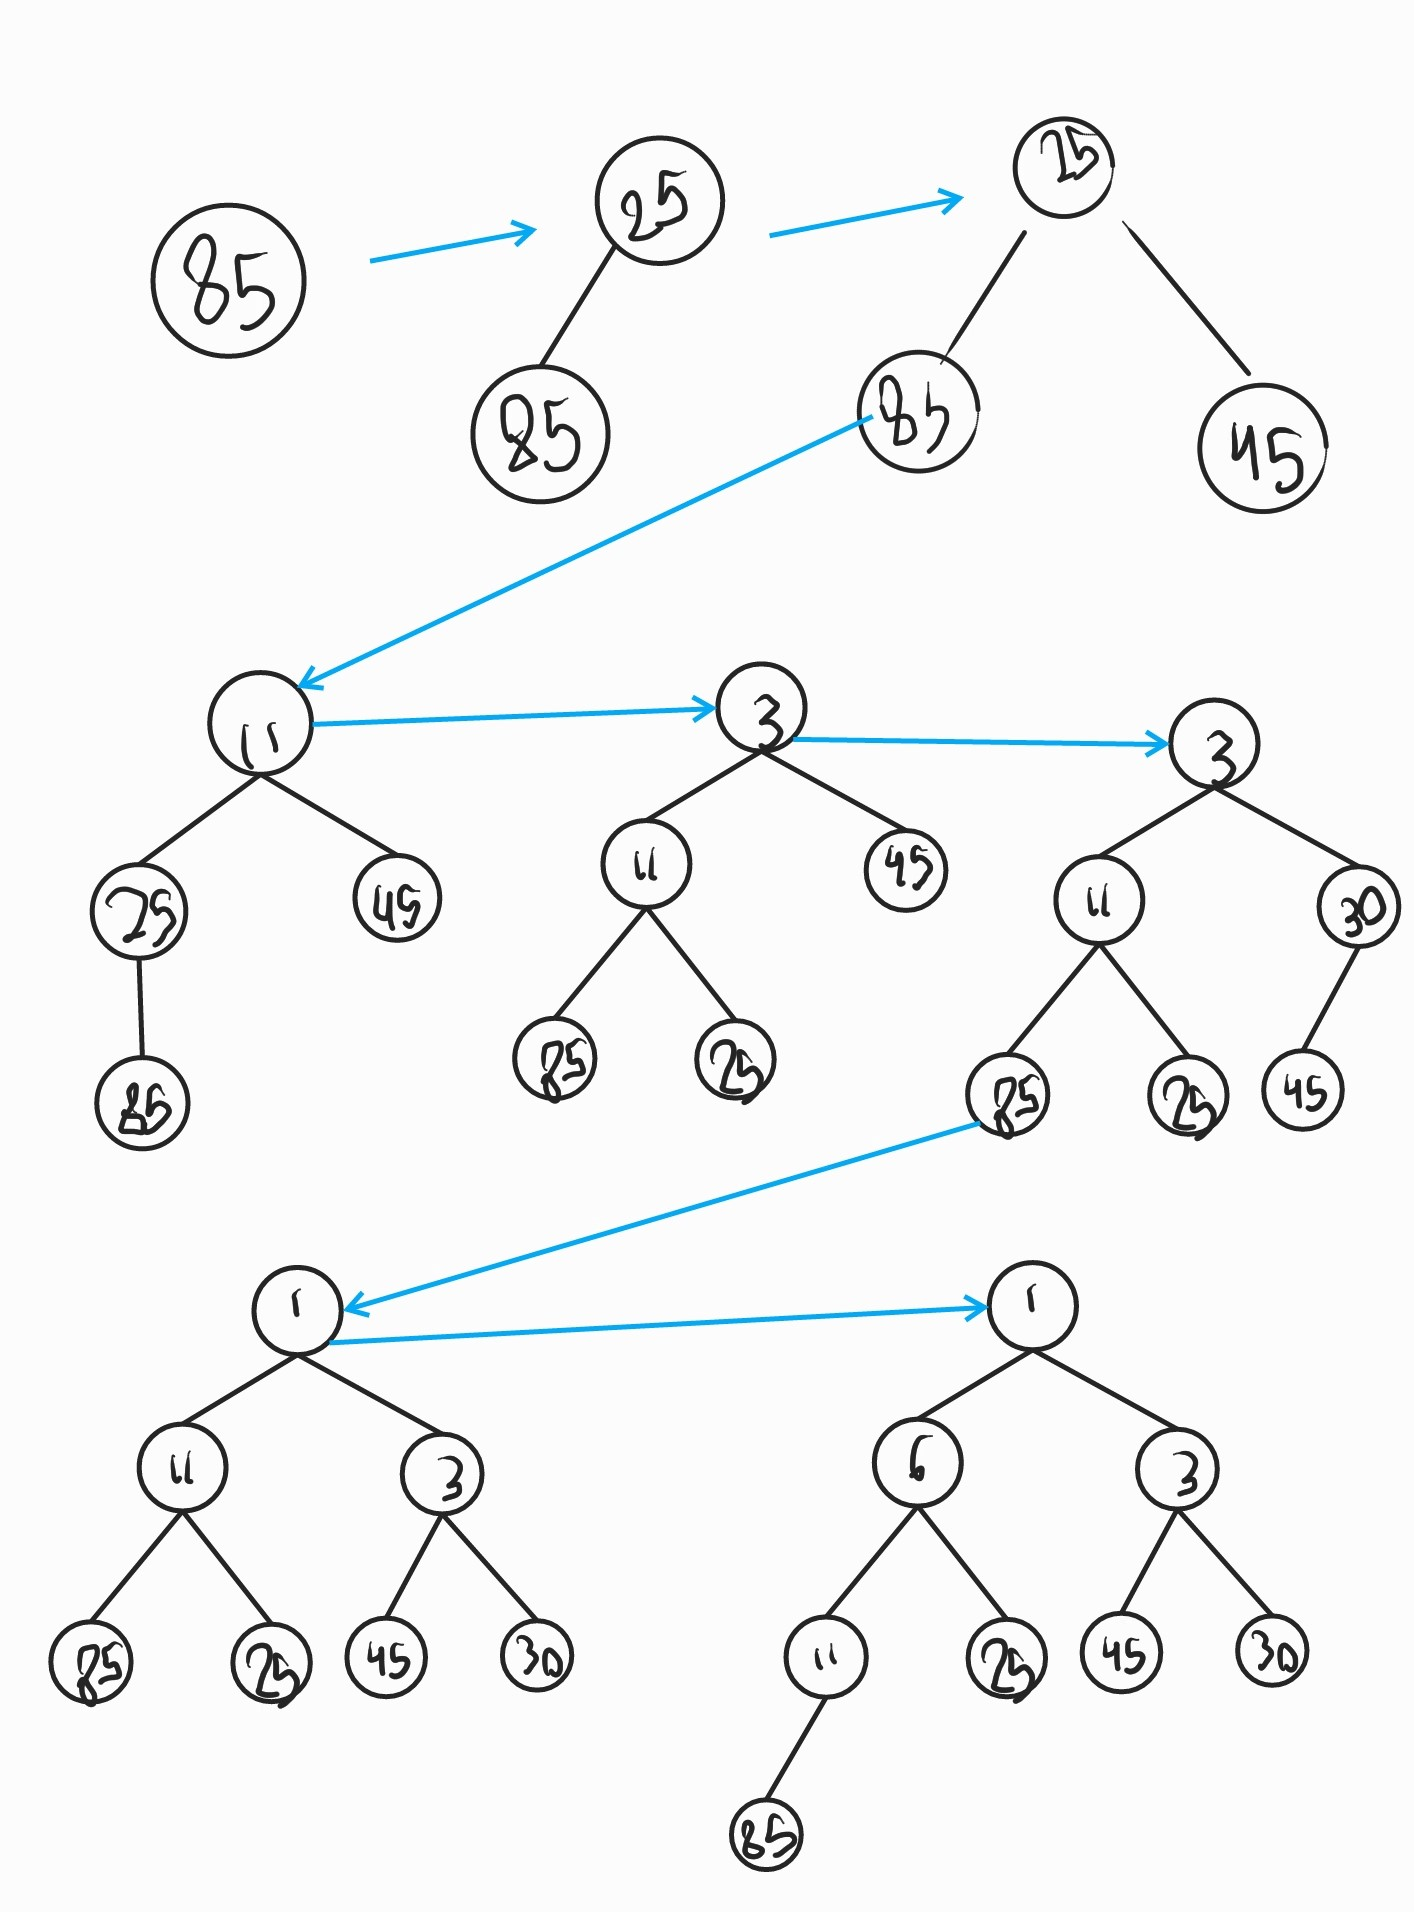
\includegraphics[scale = .1]{Images/Heap.jpg}
				\caption{Construcción Árbol}
			\end{figure}
			
			\begin{figure}[H]
				\centering
				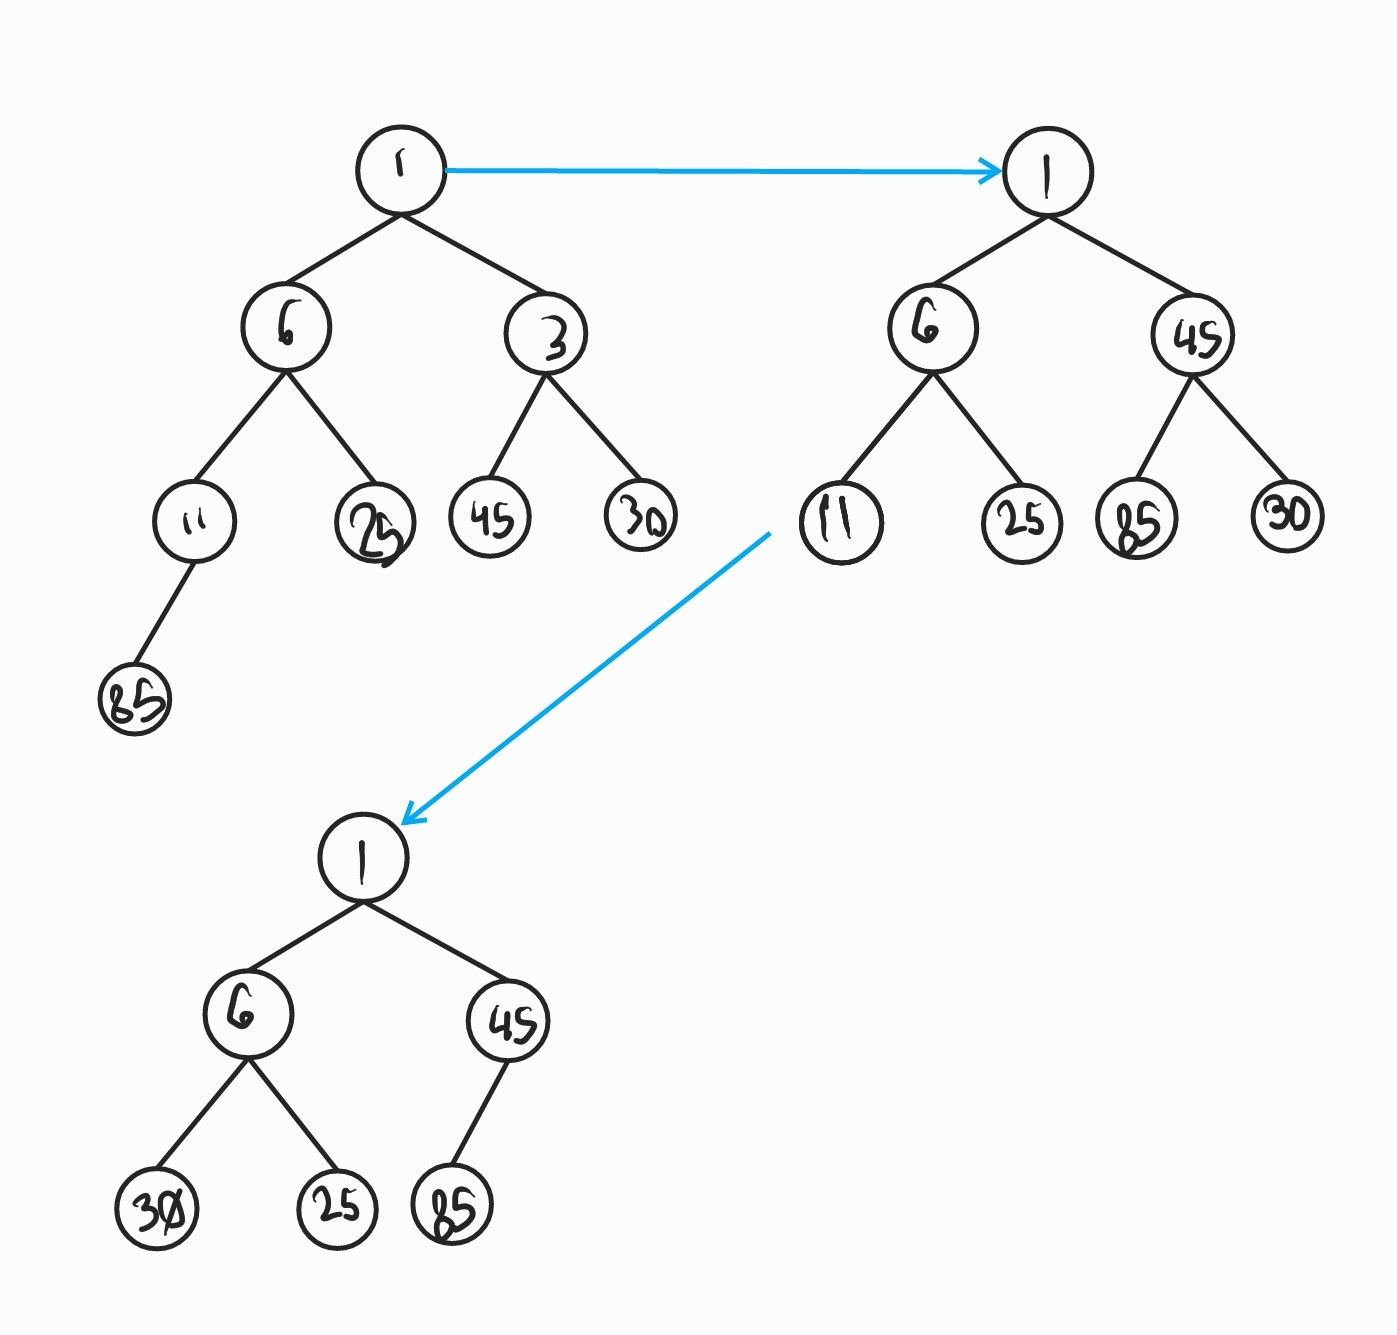
\includegraphics[scale = .1]{Images/Heap1.jpg}
				\caption{Eliminación de nodos}
			\end{figure}

		\end{multicols}

		\item Algoritmos de Ordenamiento
		
		\begin{enumerate}
			\item Es cuando un conjunto de datos no importa el orden de estos en la entrada siempre tomara el mismo número de accciones ordenarlo.
			\item InsertionSort,MergeSort,Heap-sort
			\item MergeSort,Heap-Sort
			\item InsertionSort,Heap-Sort
			\item MergeSort,QuickSort
		\end{enumerate}

		\item Tipos de Algoritmos de Ordenamiento
		
		\begin{enumerate}
			\item Merge sort
			\item Selection sort
			\item Quicksort
			\item Insertion sort
			\item Heapsort
		\end{enumerate}

		\begin{figure}[H]
			\centering
			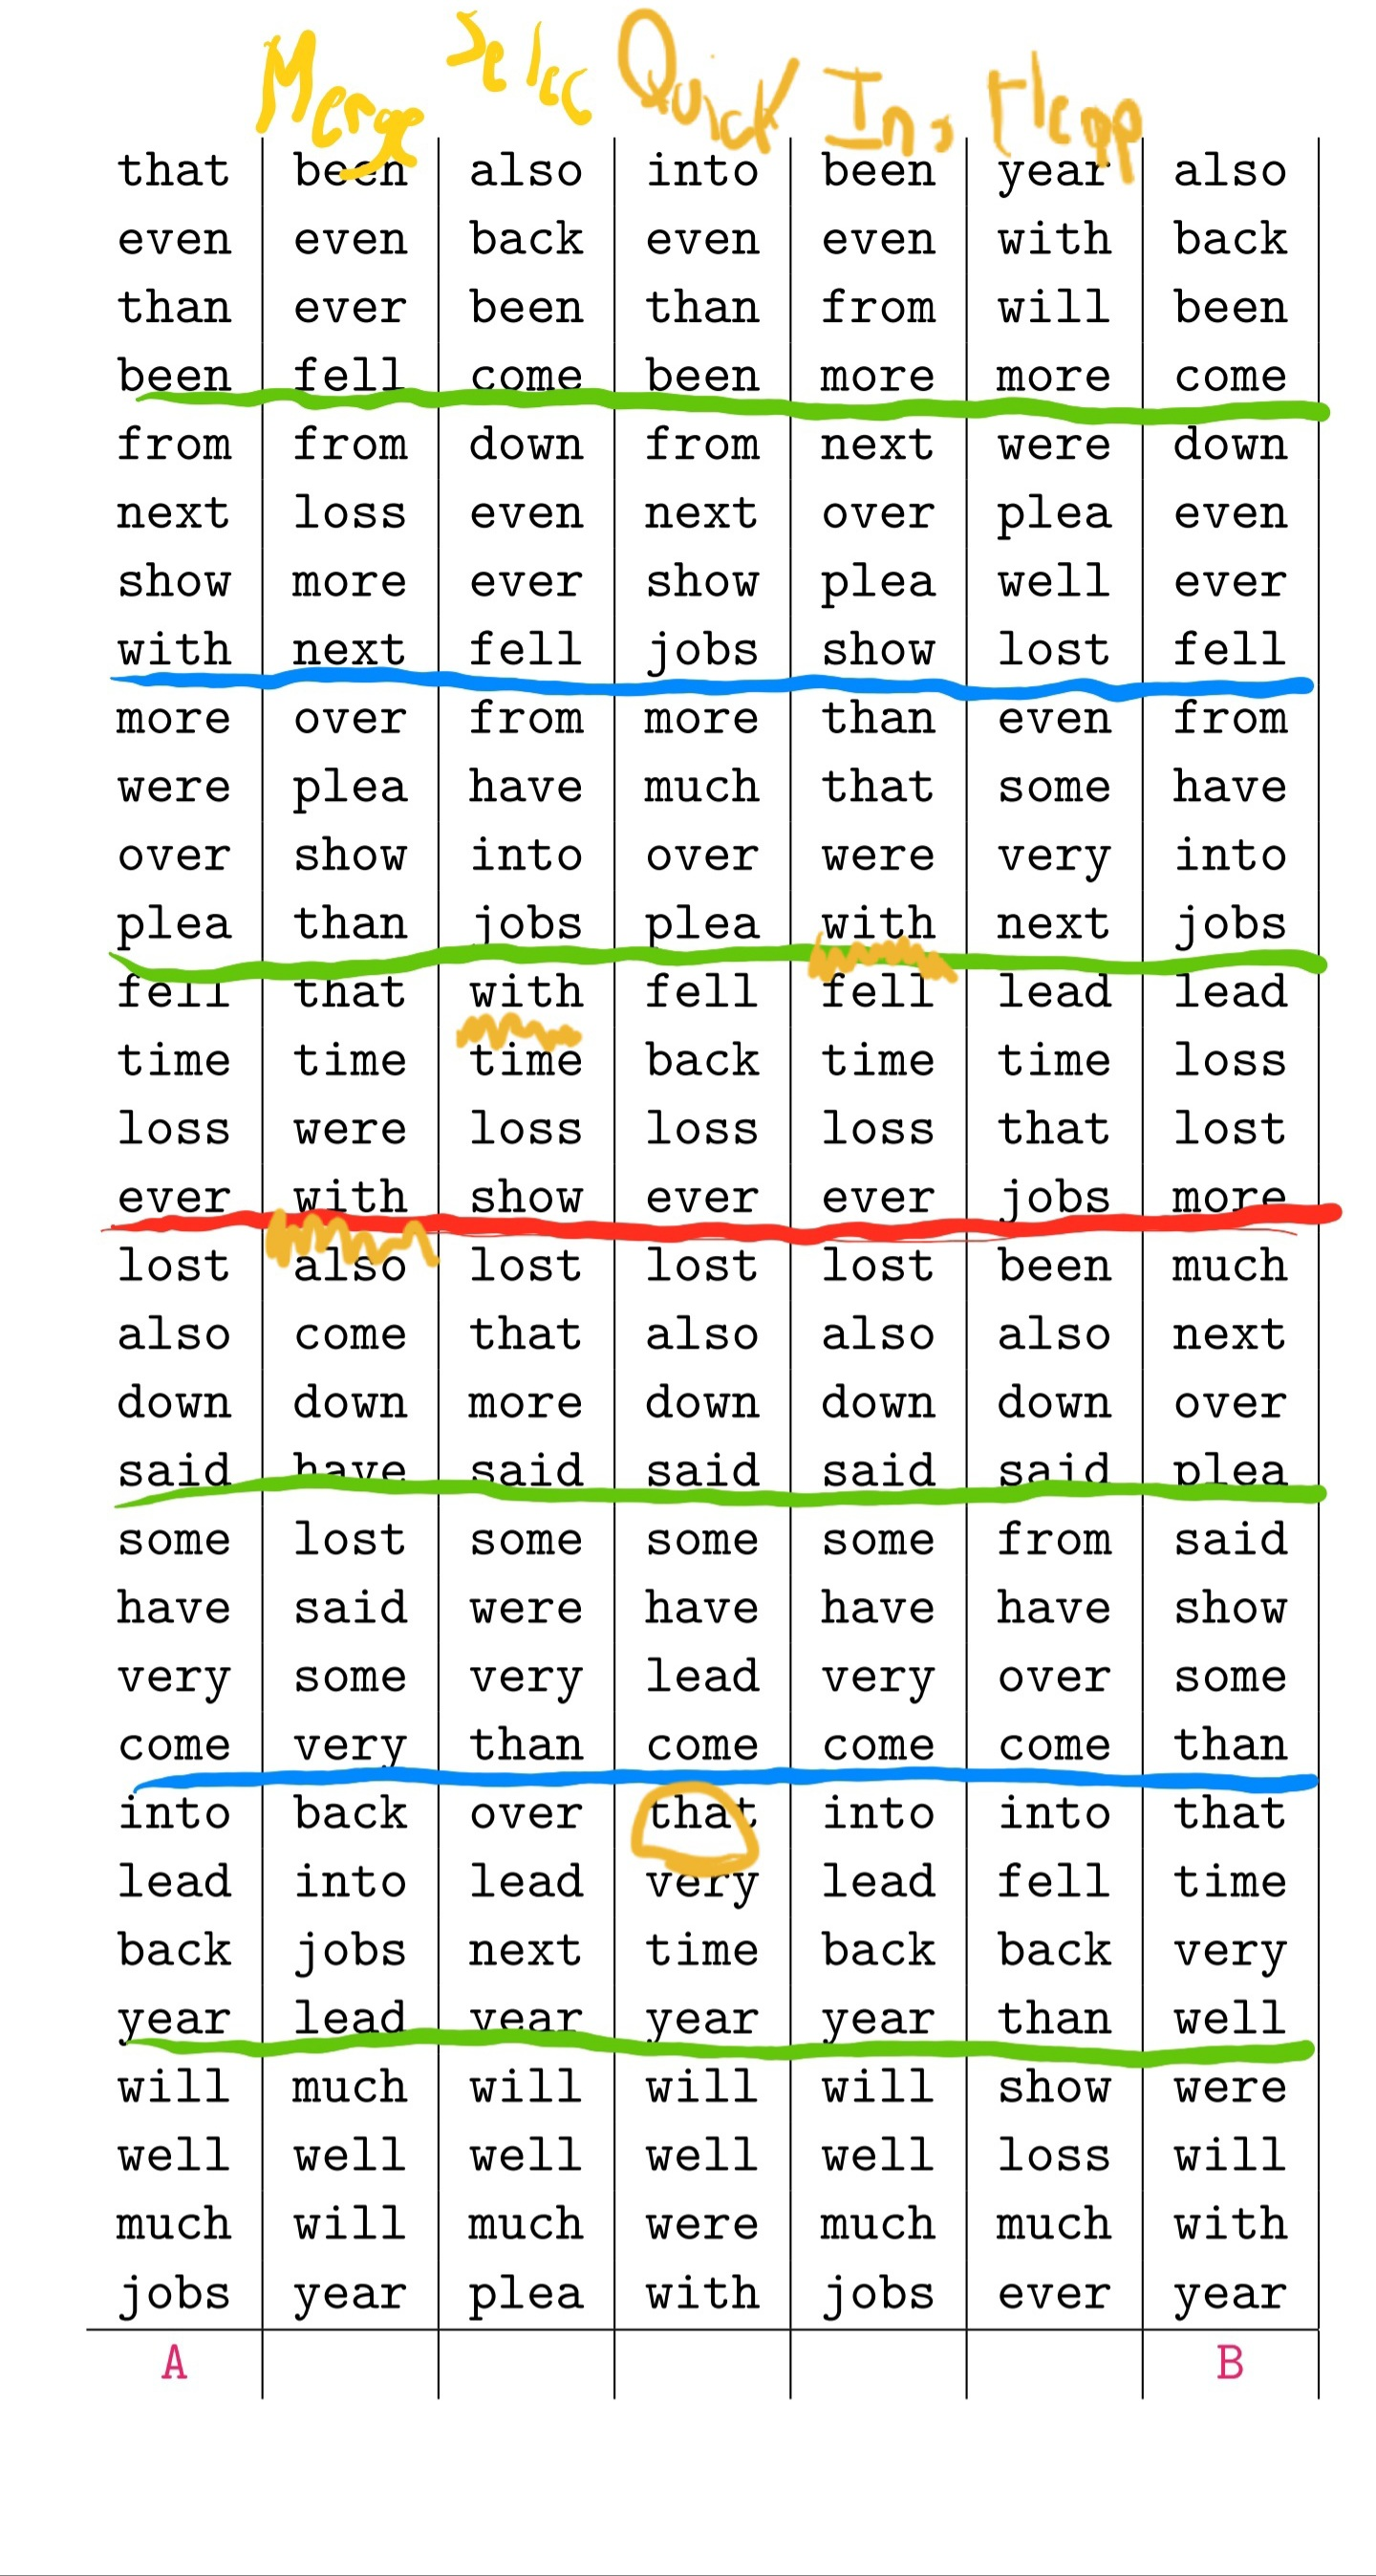
\includegraphics[scale=.06]{Images/Sort.jpg}
		\end{figure}

	\end{enumerate}
	
\end{document}
